\chapter{Related Work}
\label{chapter:ch2}
In this chapter we will thoroughly discuss works related to the current thesis. Firstly we explore computer vision model architectures that are used as feature extractors\cite{pre_trained}, namely Vision Transformers\cite{vit}, Convolutional Neural Networks\cite{lenet}, Residual Networks\cite{resnet} and Wide Residual Networks\cite{wideresnet}. We will investigate the differences between aforementioned architectures in order to bring attention to their drastic difference in performance as feature extractors for industrial anomaly detection models. Second, we will delve into the topic of unsupervised\cite{unsupervised_survey} and self-supervised\cite{self_supervised_survey} learning specifically. The comprehensive analysis of self-supervised learning model DINO\cite{dino}, which we utilize broadly in this work due to the unlabeled nature of a dataset extracted with our method, will be provided. Thereafter, a detailed discussion on Industrial Anomaly Detection will be provided\cite{iad_survey}. This section will also present the challenges the field faces with the scarcity of diverse training data and the need of Unsupervised Industrial Anomaly Detection models. Lastly, we analyze is PatchCore models which uses saves extracted features in a memory bank.

\section{Vision Transformer}
\label{vit}
Introduction of Vision Transformers\cite{vit} have presented a significantly different approach to computer vision tasks, where the standard approach of using convolutional neural networks\cite{lenet} have been replaced by transformer\cite{transformer} architecture. Until the point of introduction of vision transformers, transformer architecture was commonly used for natural language processing\cite{natural_language}\cite{transformer} tasks. Transformer architecture leverages self-attention\cite{transformer} mechanism which has the ability to capture relationship between all parts of data with each other. In case of Vision Transformers, self-attention mechanism is able to capture the global context of the image rather than focusing on local features\cite{vit} as CNN\cite{lenet} filters do.

One of the main challenges when it comes to utilizing transformer architecture on visual data, is that it does not have the ability to capture spatial information as the traditional CNN\cite{lenet} models do. Moreover, transformers are originally equipped to work with sequential data like a stream of words\cite{transformer} which images are not. In order to make images a viable input for transformer, the image is split into constant size patches which are then embedded with positional encodings saving crucial spatial information\cite{vit}. Transformer evaluates the relationships between all the patches using the self-attention mechanism\cite{transformer}. Thereafter, output from the transformer is used as an input for classification feed-forward network\cite{vit}. In the case of Industrial Anomaly Detection\cite{iad_survey}, output from each transformer layer can be used as extracted features in anomaly detection models\cite{pre_trained_iad}. The diagram of the ViT architecture is shown on the figure \ref{fig:vit}.

\begin{figure}[t]
	\begin{center}
		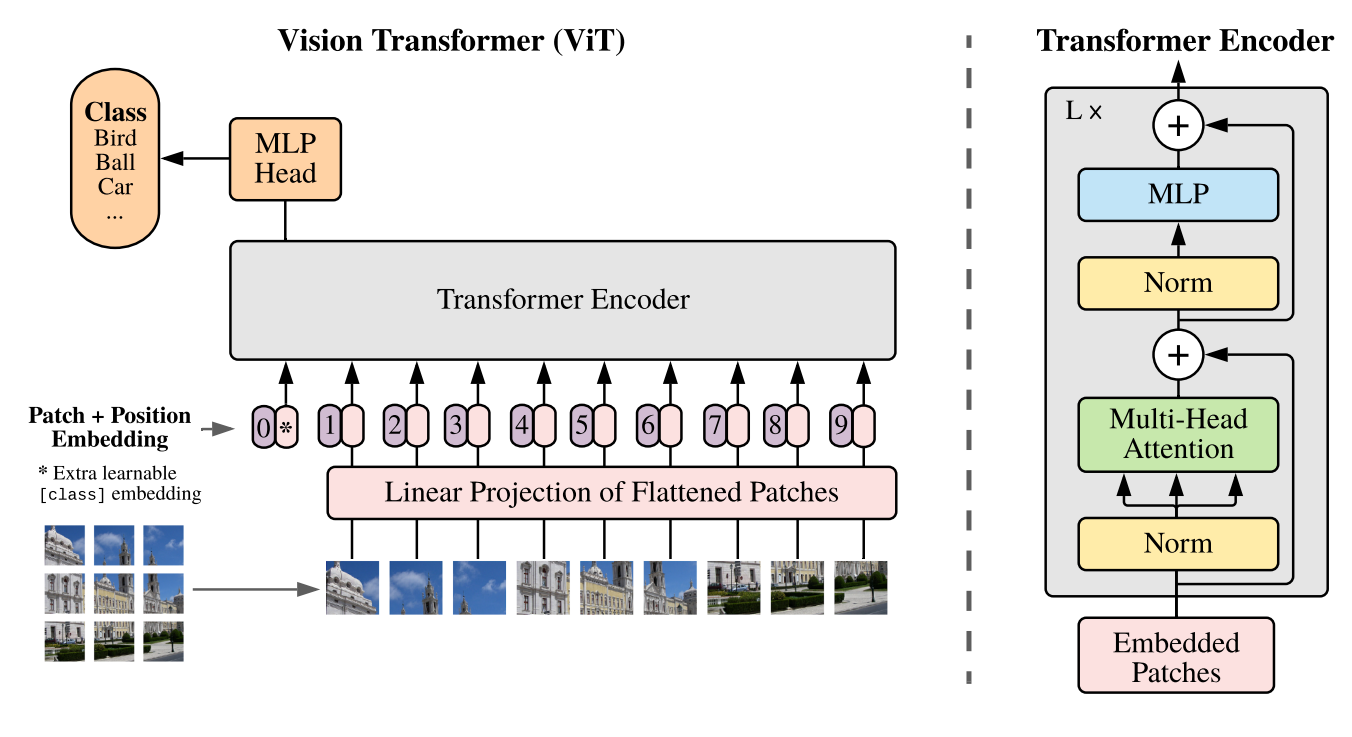
\includegraphics[width=0.8\linewidth]{Chapter_2/vit.png}
	\end{center}
	\caption{Vision Transformer model which uses the Transformer encoder shown on the right to capture meaningful features from the images. The images have to be split into patches to transform them into a sequential data in order to make them to be able to be captured by Transformers\cite{transformer}. \cite{vit}}
	\label{fig:vit}
\end{figure}

In the recent years Vision Transformers have been used extensively in self-supervised learning models\cite{dino}\cite{self_supervised_survey}. The prevalence of Vision Transformers in self-supervised learning can be explained by the ability of them to utilize the global context of images, which allows them to be able to extract high quality features from unlabeled data\cite{vit}. Methods like contrastive learning proved\cite{contrastive} to be very efficient when used in combination with Vision Transformers\cite{vit_contrastive} especially.

\section{Convolutional Neural Networks}
\label{cnn}
For many years Convolutional Neural Networks have been the main architecture in the field of image processing due to their ability to capture spatial hierarchical features\cite{cnn_survey}. They have been used efficiently in tasks such as image classification, semantic segmentation and object detection. When this architecture was introduced by Yann LeCunn and colleagues in 1980\cite{lenet}, it revolutionized the field showing significant increase in accuracy over the methods that used to be prevalent.

The main novelty that Convolutional Neural Networks introduced were the convolutional and pooling layers of the network\cite{lenet}. Convolutional layer performs a "convolution" operation using kernels on the input image or, in the later layers, on the features extracted by the filters of the previous layer\cite{lenet}. In the first layers, local features are captured by convolution and in the later layers, pooling operation is performed, which serves as dimensionality reduction and extraction of global features from local ones. In more recent models convolution and pooling layers are also followed by normalization layers, which stabilizes and speeds up the training process\cite{batchnorm}. Between each layers of the model, some non-linearity function, which is usually ReLU activation function, is used to allow the model to learn to generalize more complex structures of data. Generally, the final stage of CNN\cite{lenet} architectures consist of fully-connected layers that maps the learned features to specific classes. To have a better understanding of the architecture please look at the figure \ref{fig:cnn}

\begin{figure}[t]
	\begin{center}
		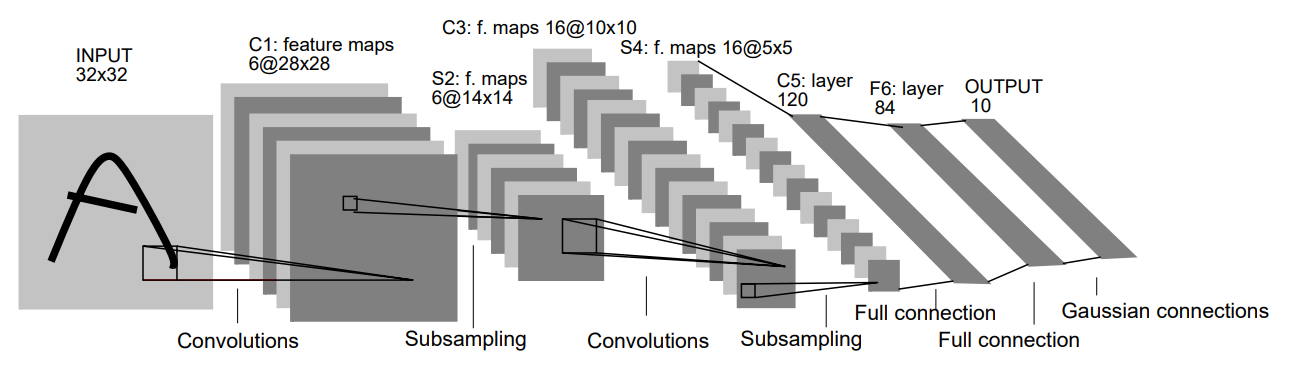
\includegraphics[width=1.0\linewidth]{Chapter_2/cnn.png}
	\end{center}
	\caption{Convolutional Neural Network consisting of convolution and subsampling layers. Its architecture allows for the efficient capture of spatial features, which can explain its prominence in anomaly detection models.\cite{lenet}}
	\label{fig:cnn}
\end{figure}

In spite of the fact that Vision Transformers\cite{vit} have been emerging as the competitor to the CNN\cite{lenet} architectures, CNN\cite{lenet} architectures still stand as the preferable option in certain specific cases, Industrial Anomaly Detection\cite{iad_survey} being one of them. The ability of CNNs to capture local features and spatial hierarchies with high accuracy, can contribute to their efficiency as feature extractors in IAD models.

\subsection{Residual Networks}
\label{resnet}
Residual Neural Network\cite{resnet} architectures are the subset of CNNs\cite{lenet} that are designed for deep learning scenarios and address one of the main challenges of training deep neural networks. The ResNet model, which is most commonly used Residual Network model, presented a concept of skip connections which is a connection between layers that skips some layers(usually one) in between\cite{resnet}. This new addition allows models to have hundreds of layers, which was impossible due to the vanishing gradients problem.

The usual ResNet\cite{resnet} model consists of residual blocks that have a skip connection at the input connecting directly to the output of the block. Skip connection(figure \ref{fig:res_block}) facilitates the model to learn a residual mapping F(x) = H(x) - x, instead of the direct H(x) mapping from the input x, which allows the model to learn residuals or differences, rather than the one-to-one mapping\cite{resnet}. Each residual block contains multiple convolutional layers and activation layers. In most of the ResNet implementations, such as ResNet50\cite{resnet}, a bottleneck residual connection is used which consists of a 3x3 convolution layers in between two 1x1 convolution layers. All the innovation present in ResNet\cite{resnet} architecture allows for the training of multi layer deep models without the vanishing gradients problem and preserving the learned features across layers.

\begin{figure}[t]
	\begin{center}
		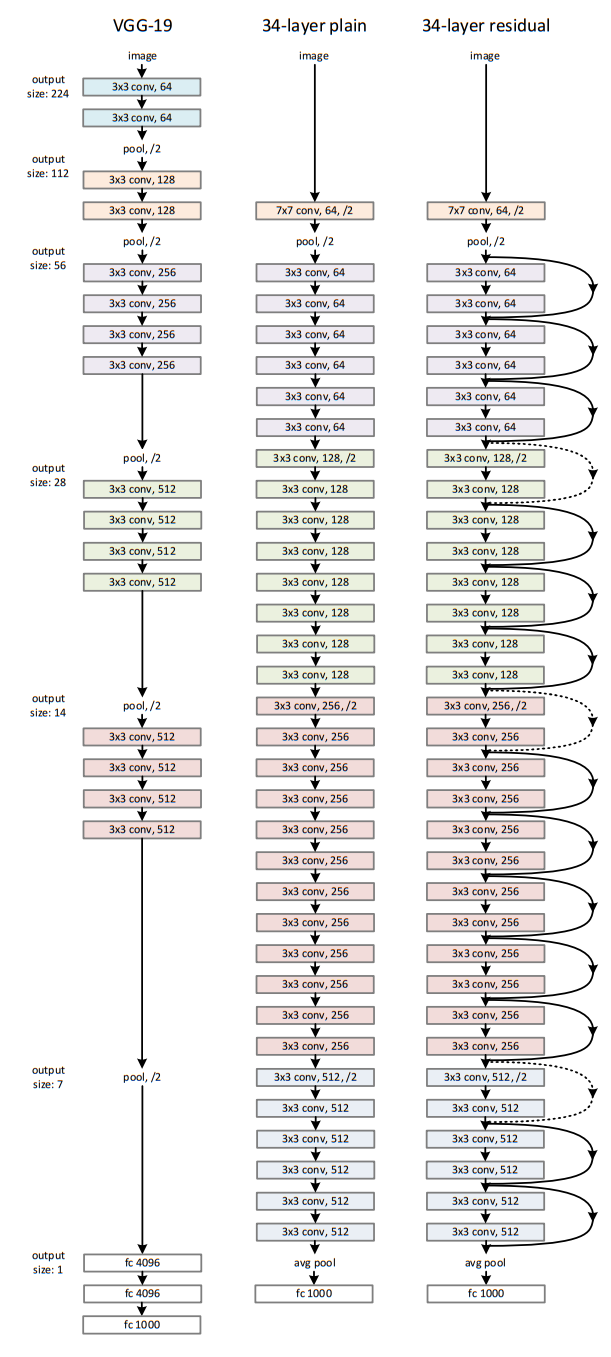
\includegraphics[width=0.5\linewidth]{Chapter_2/resnet.png}
	\end{center}
	\caption{Residual block that allows for the assembly of deep computer vision models.\cite{resnet}}
	\label{fig:res_block}
\end{figure}

ResNet\cite{resnet} emerged as a dominant model to be used as feature extractors in industrial anomaly detection models. This choice is driven mainly by empirical evidence to their efficiency. However, we can also see that in ResNet\cite{resnet} models the advantages of CNNs, such as capturing local features and spatial hierarchies, are amplified by allowing us to train larger size CNN models. Advantages which might make CNNs a preferable choice as feature extractors for IAD models.

\subsection{Wide Residual Neural Networks}
\label{wideresnet}
WideResNet, which is the most prominent Wide Residual Neural Network model\cite{wideresnet} is enhancement upon the regular ResNet architecture, which focus on increasing the width of the model instead of the depth. The main point of this improvement is in the residual blocks where the channels of convolutions are increase by some factor(figure \ref{fig:wide_resnet}), allowing the model to have increase representational capacity while maintaining the ability to train deep networks\cite{wideresnet}. Increased channel size also allows Wide ResNets to have improved gradient flow which enhances the models capability to learn from large complex datasets. The enhancements allow Wide ResNets to have higher capacity to learn fine-grained details which makes this type of architecture a suitable choice for usage as feature extractors in IAD models.

\begin{figure}[t]
	\begin{center}
		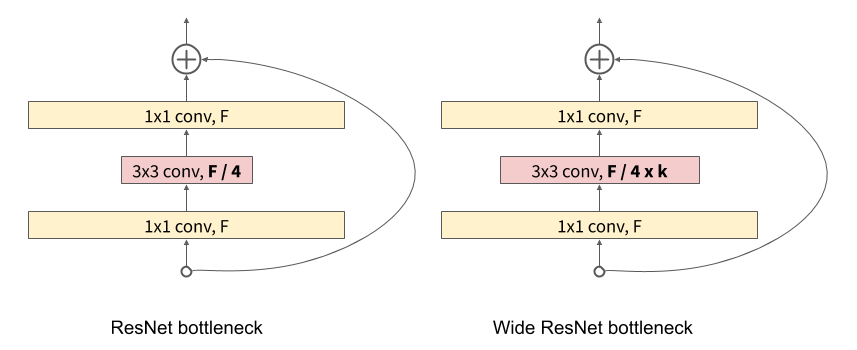
\includegraphics[width=1.0\linewidth]{Chapter_2/wide_resnet.png}
	\end{center}
	\caption{Difference between Wide Residual Block and standard residual block, where the WideResNet has the width increase by the factor of k\cite{wideresnet}\cite{pytorch_wide}}
	\label{fig:wide_resnet}
\end{figure}

\section{Unsupervised Learning}
\label{usupervised learning}
To generate feature spaces suitable for industrial anomaly detection tasks, it is beneficial to use multiple available, large scale, unlabeled image datasets. One of the many Unsupervised Learning techniques will allow us to effectively extract features from unlabeled datasets. Unsupervised Learning refers to the variant of machine learning algorithms where the models is trained to learn patterns in the data itself, instead of overt output labels like in supervised learning\cite{unsupervised_survey}. Unsupervised Learning models in their process leverage such architectures as autoencoders which work by first transforming the data into a compressed representation and then learning to restore the input, generative adversarial networks which train two competing models discriminator and a generator, clusterization algorithms which separates the input into clusters using algorithms like k-NN, contrastive learning which learns features by comparing input data\cite{unsupervised_survey}. 

\subsection{Self-supervised Learning}
\label{self-supervised learning}
Self-supervised learning are a subset of unsupervised learning models in that, they also designed to learn from unlabeled data but unlike unsupervised learning models that learn representation from the data directly, self-supervised learning first assigns "labels" or "tasks" on unlabeled data and learns to fit the generated labels or complete the generated tasks in order to extract hidden structures and patterns from the provided input\cite{self_supervised_survey}. Therefore, self-supervised learning serves as the middle ground between unsupervised and supervised learning, in an attempt to leverage the advantages of supervised learning in an unsupervised setting. Over the recent years, self-supervised learning models proved to be very efficient method of unsupervised learning, allowing to train models that can perform with high accuracy on multiple tasks after the task specific fine-tuning process\cite{self_supervised_survey}.

As have been stated the key component of self-supervised learning is the generation of assisting tasks based on the training data\cite{self_supervised_survey}\cite{dino}. An example for the types of tasks that might be generated can be, predicting various transformations applied on the image\cite{dino} or drawing in the random missing patches of the image\cite{self_patch}. By training to accomplish this tasks, self-supervised model learn the patterns that inherently exist in the data, extracting valuable features in the process. This mode of learning can be utilized to generate feature spaces suitable for the task of industrial anomaly detection from large scale unlabeled datasets. Indeed, we use one of the most robust self-supervised learning models DINO\cite{dino} in this work.

\subsection{DINO model}
\label{dino}
DINO(from distillation with no labels) is a robust self-supervised learning model that was introduced by Facebook AI team that uses enhanced knowledge distillation pipeline to learn useful representations from an unlabeled large image datasets\cite{dino}. The model achieves high accuracy on top-1 classification task on the ImageNet dataset, specifically 79.1 percent when training the model ViT-S/14 and higher 82.1\% when used with the ViT-B/14 model\cite{dino}. DINO models ability to train both Vision Transformer and CNN based model and its high efficiency makes the model an excellent choice for the purposes of this thesis.

In its training process DINO utilizes the teacher-student architecture where student is trained to align its output to the output of the teacher model\cite{dino}. Both student and teacher models trained using the same model architecture but using different parameters. The key point of the DINO model is that the teacher model is trained using the EMA - exponential moving average of the student model in order to guarantee the stability during training\cite{dion}. Training process itself consists of passing an input image with random transformations picked from a constant set of transformations, to teacher and student models and adjusting the student models output to the teacher models output using cross-entropy loss function. During such a training process, the student model learn invariant and meaningful features from the input\cite{dino}. The architecture is shown in the figure \ref{fig:dino}

\begin{figure}[t]
	\begin{center}
		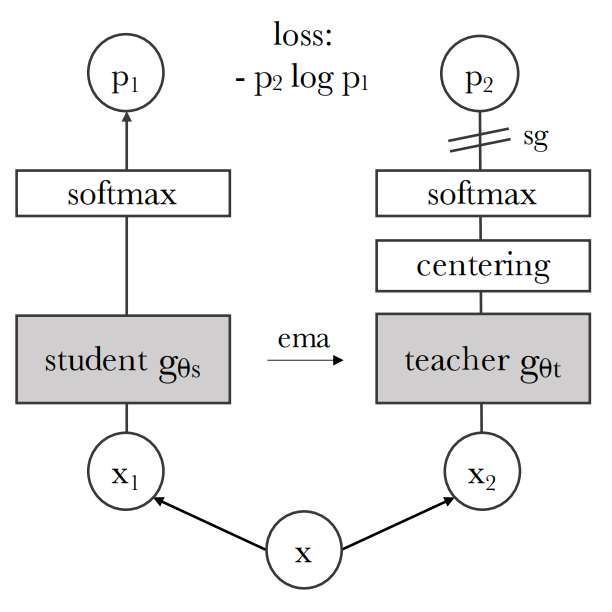
\includegraphics[width=0.5\linewidth]{Chapter_2/dino.png}
	\end{center}
	\caption{architecture of a DINO model consisting of a student and a teacher model.\cite{dino}}
	\label{fig:dino}
\end{figure}

\section{Industrial Anomaly Detection}
\label{iad}
Industrial Anomaly Detection has become the irreplaceable part of various manufacturing processes, allowing to detect any deviations from standards of manufacturing and preventing defective products from potentially reaching the output\cite{iad_survey}. Anomalies of varying kind expected to happen in every industrial processes due to different reasons like, wear and tear, software errors and malfunction of devices. Industrial Anomaly Detection methods allow us monitor the manufacturing pipeline and to anticipate such defects, followed with swift corrections\cite{iad_survey}. This allows for increased stability of manufacturing, improved quality control, mediating costly defects, minimizing downtime and enhancing efficiency. For the visual explanation, refer to \ref{fig:iad}

\begin{figure}[t]
	\begin{center}
		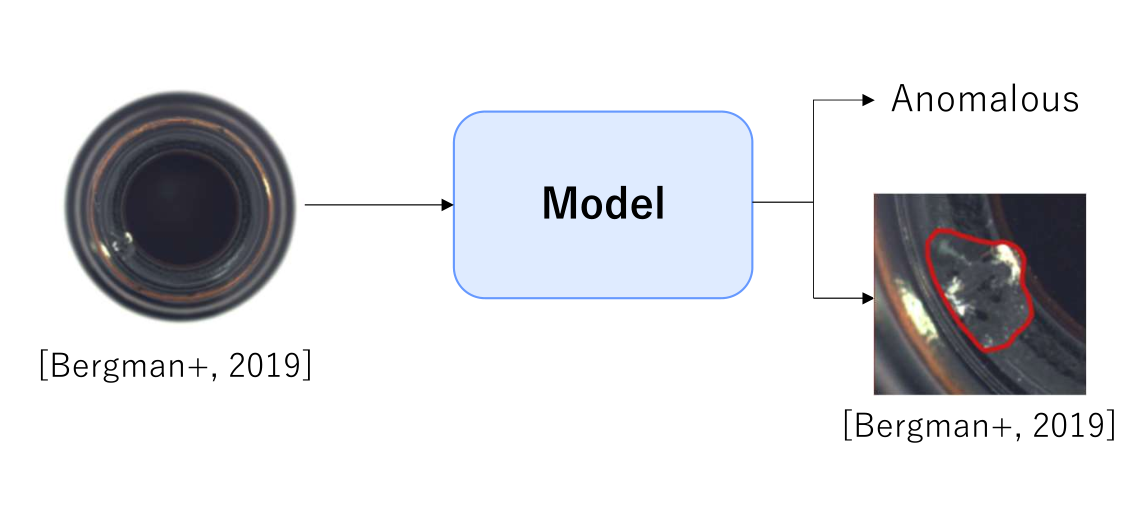
\includegraphics[width=0.8\linewidth]{Chapter_2/iad.png}
	\end{center}
	\caption{The process of Industrail Anomaly Detection}
	\label{fig:iad}
\end{figure}

Contemporary Industrial Anomaly Detection methods heavily rely on deep learning computer vision models. Variety of computer vision models like convolutional neural networks, vision transformers and autoencoders can be utilized to efficiently implement industrial anomaly detection in real use case scenarios where data from visual sensors such as cameras\cite{iad_survey}. These models posses the ability to learn complex visual representation from high-dimensional imagery data, allowing IAD tasks to be performed with high accuracy and reliability. Over the recent years the field of Industrial Anomaly Detection witnessed a lot of improvements, especially in the field of Unsupervised Industrial Anomaly Detection where there is a scarcity of anomalous data. 

\clearpage
\subsection{Unsupervised Industrial Anomaly Detection}
\label{unsupervised iad}
Unsupervised Industrial Anomaly Detection leverage unsupervised deep learning techniques in order to learn any deviations from the nominal patterns it the provided input. In IAD field unsupervised learning is vital because labeled anomalous images are extremely scarce or non-existent\cite{mvtecad}\cite{realnet}. There are multiple types of architectures that can be engaged to implement unsupervisded iad models, including architectures like autoencoders\cite{realnet}, clustering\cite{patchcore} and various statistical techniques are common to be used\cite{uiad_survey}. As an example, PatchCore\cite{patchcore} model uses memory-bank approach opting to save features extracted by pre-trained backbone model with some aggregation operations while on the inference performing kNN over the saved features and extracted features of the test sample. Another model called SimpleNet trains a discriminator with synthetically generated anomalies on the features of the nominal samples. There are also reconstruction based models like RealNet\cite{realnet} which utilized auto-encoders on the layers of the pre-trained feature extractor model. In this thesis, we use these three models to test different feature spaces on. Refer to figure \ref{fig:uiad} for the visual representation of the Unsupervised IAD process.

\begin{figure}[t]
	\begin{center}
		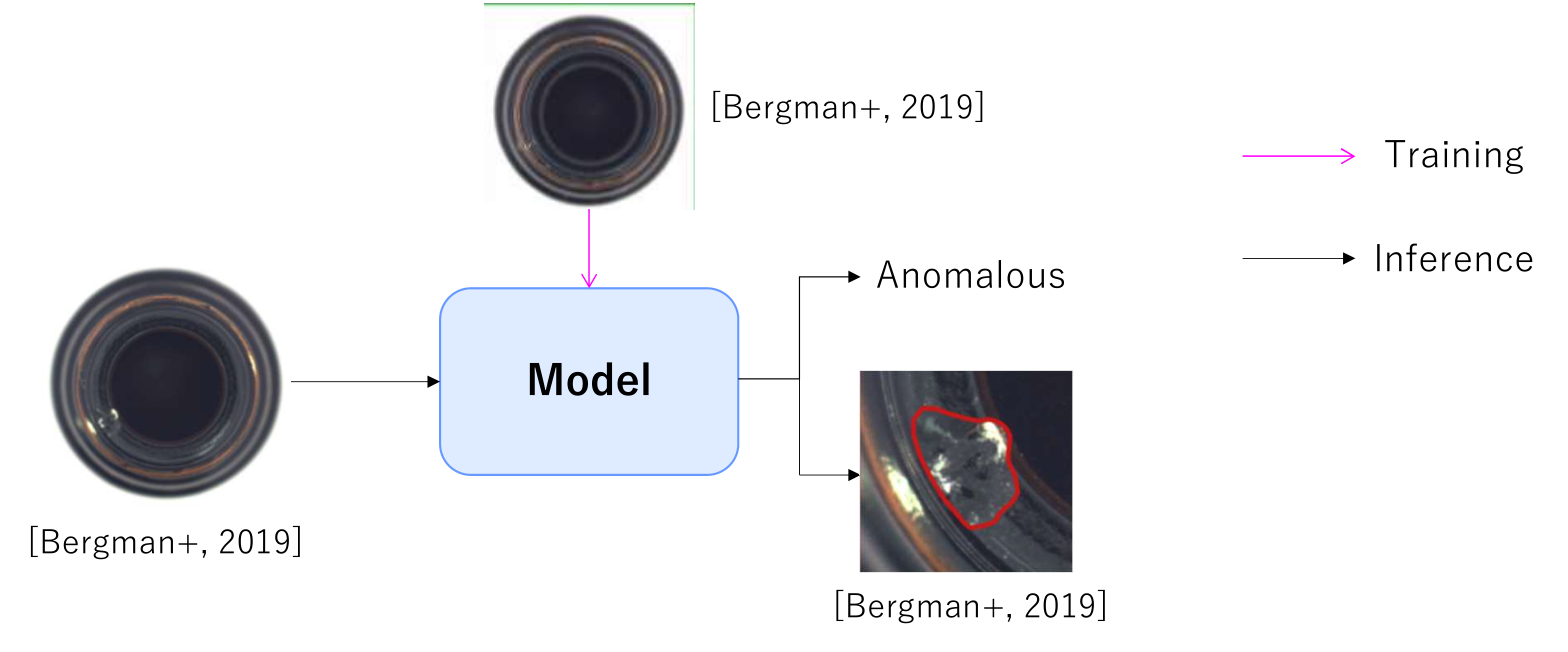
\includegraphics[width=0.8\linewidth]{Chapter_2/uiad.png}
	\end{center}
	\caption{Unsupervised anomaly detection pipeline.}
	\label{fig:uiad}
\end{figure}

\clearpage
\subsection{PatchCore}
\label{patchcore}
The PatchCore\cite{patchcore} industrial detection model is designed to excel in identifying anomalies in visual data for industrial applications. The methodology behind PatchCore involves several key steps. Initially, the model utilizes pre-trained convolutional neural networks (CNNs) to extract high-dimensional feature representations from input images\cite{patchcore}. These features are then divided into smaller patches, which are processed individually. The core idea of PatchCore is to leverage these patches for local anomaly detection, ensuring that even small, subtle defects can be detected\cite{patchcore}. The model applies an anomaly scoring mechanism to each patch, comparing it to a reference distribution of normal patches derived from a training dataset\cite{patchcore}. This scoring helps in distinguishing between normal and anomalous regions within an image. Additionally, PatchCore incorporates a memory bank of normal patches, enabling efficient and accurate comparison during inference\cite{patchcore}. By focusing on local patches rather than the entire image, PatchCore enhances the precision and reliability of anomaly detection, making it well-suited for diverse industrial inspection tasks where fine-grained anomalies are critical to detect\cite{patchcore}. Refer to figure \ref{fig:patchcore} for the visual representation of the models architecture.

\section{MVTechAD}
\label{mvtech}
The MVTec Anomaly Detection (MVTec AD) dataset is a comprehensive benchmark specifically designed for evaluating anomaly detection methods in industrial inspection\cite{mvtecad}. It comprises over 5,000 high-resolution images across fifteen different object and texture categories, each containing defect-free training images and a test set with various types of defects\cite{mvtecad}. The dataset provides pixel-precise annotations of all anomalies, enabling precise evaluation and comparison of different anomaly detection techniques. MVTec AD is widely used in the research community to advance and validate new methods, ensuring they are robust and effective for real-world industrial applications. Samples from the dataset are displayed in the figure \ref{fig:mvtec}.

\begin{figure}[t]
	\begin{center}
		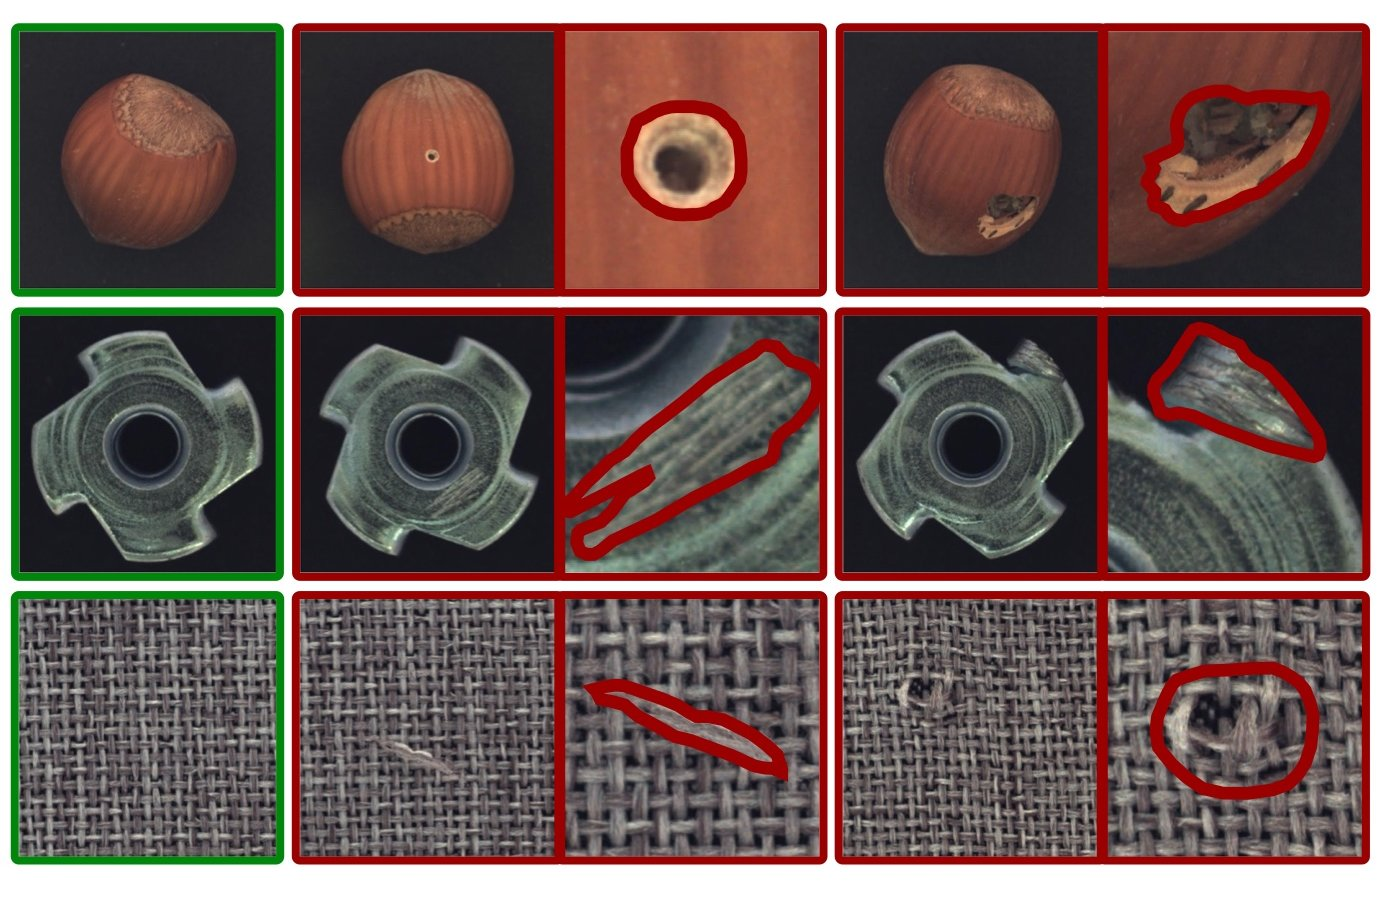
\includegraphics[width=0.7\linewidth]{Chapter_2/mvtec.jpg}
	\end{center}
	\caption{Samples from MVTech dataset.\cite{mvtecad}}
	\label{fig:mvtec}
\end{figure}

